\section{SMACCMPilot: a High-Assurance Autopilot}
\label{sec:smaccmpilot}

\begin{figure}[ht!]
  \begin{center}
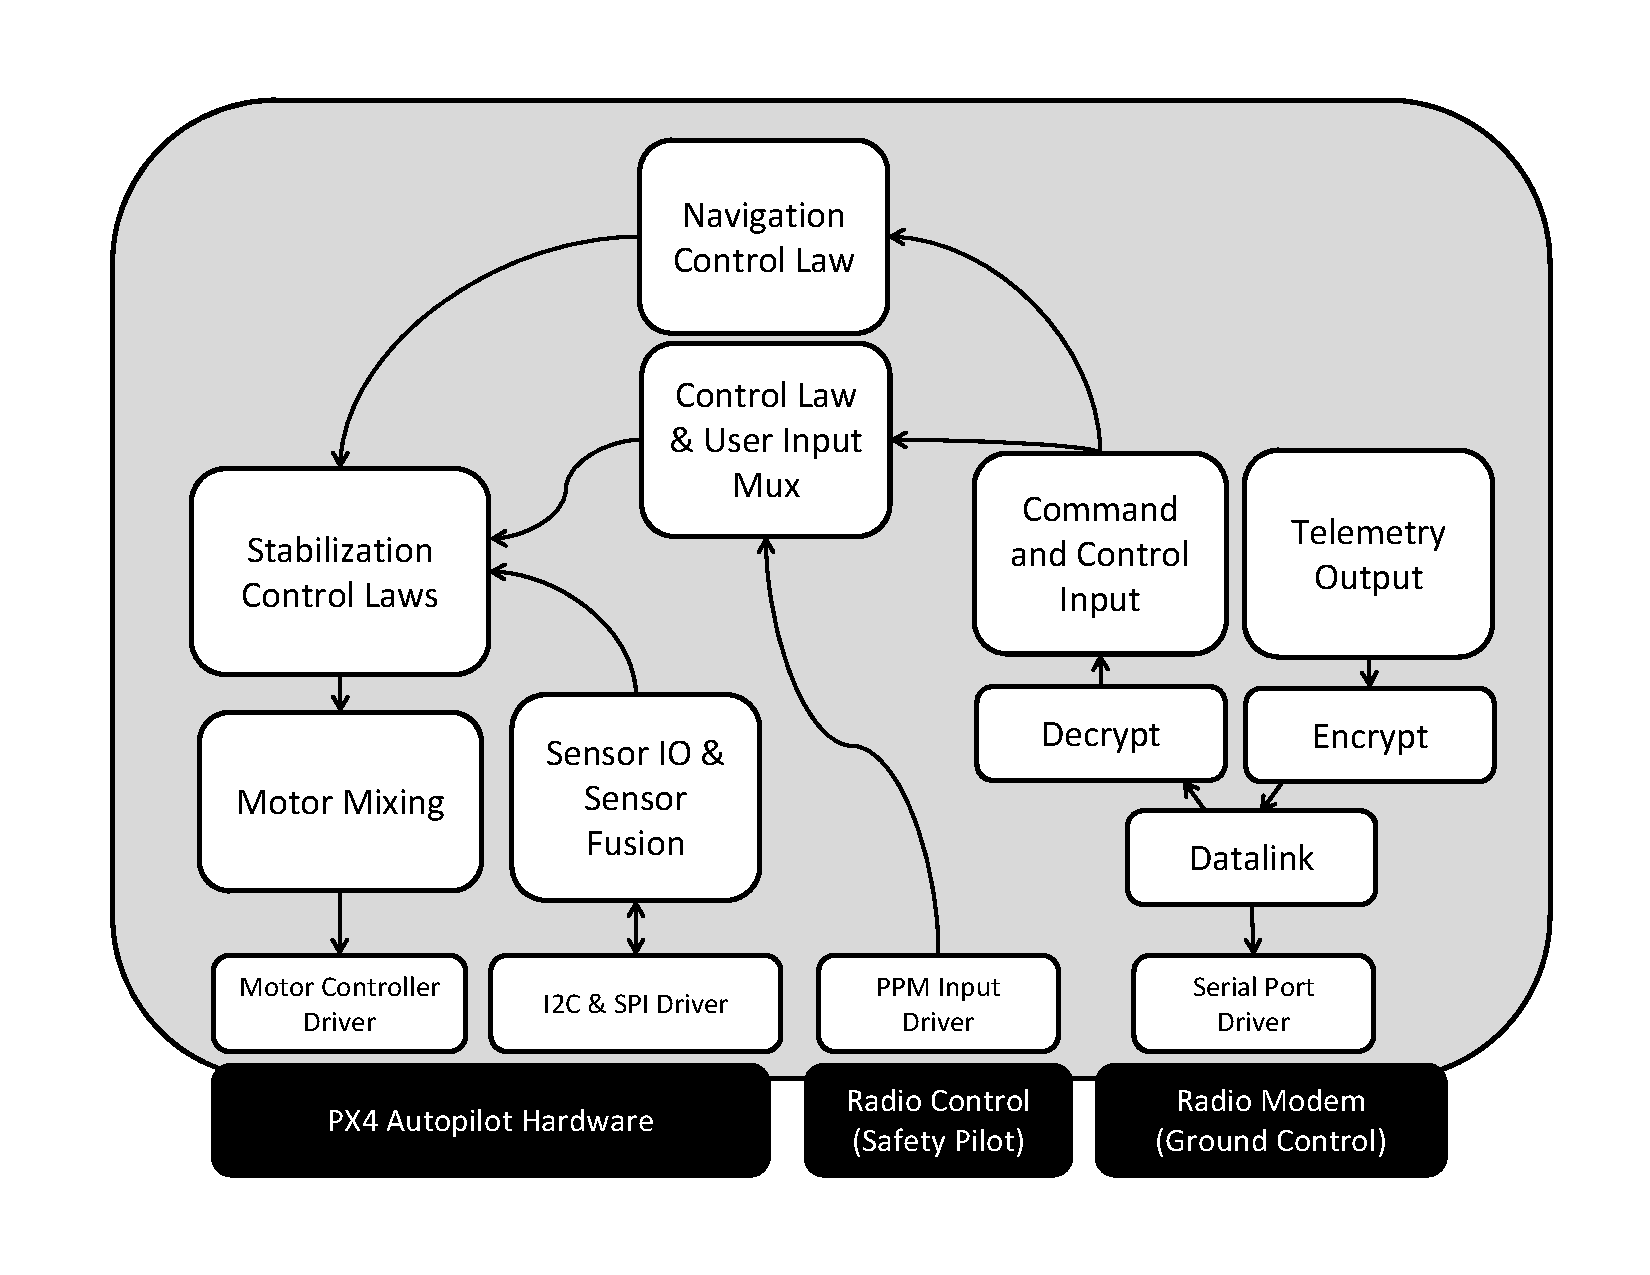
\includegraphics[width=8cm]{figures/smaccmpilot-diagram-jan14}
  \end{center}
\caption[SMACCMPilot software architecture]{Overview of SMACCMPilot
software architecture. Tasks are shown as white boxes, channels as arrows,
hardware components as black boxes.}
\label{fig:smaccmpilotSwArch}
\end{figure}

\ph{There are different font sizes in the figure}
\ph{maybe say that IC2 isn't generated yet?}
\ph{show ``commsec recovery task''?  Maybe not important...}

SMACCMPilot\ph{note BDS3 open-source, website}, the first large project
developed in the Ivory language, is a flight controller (or autopilot) for small
quadcopters. SMACCMPilot project is a high-assurance autopilot, mostly generated
from Ivory/Tower.

SMACCMPilot builds on a foundation of open source flight controller hardware
from the PX4 Autopilot project \ph{cite ethz}. The hardware platform is a
custom printed circuit board with an ARM Cortex M4 microcontroller, as well as
sensors used to determine the orientation and altitude of the vehicle.
\ph{ describe more about the individual parts of a quadcopter? }

SMACCMPilot implements all of its own low-level peripheral drivers for the
microcontroller, and higher level drivers to interface with the on-board
sensors, external motor controllers, and external radio transcievers. The flight
control software is primarily responsible for reading the sensors, estimating
the vehicle's attitude and position using sensor fusion, calculating control
outputs, and sending motor power commands to the motor controllers.  Higher
level control loops manage navigation, and an encrypted command, control, and
telemetry link interprets ground station instructions, sends system state to the
operator, and permits online tuning of control loop parameters. More details are
shown in Figure \ref{fig:smaccmpilotSwArch}.

The result is a reasonably complex piece of embedded software.  SMACCMPilot has
30 tasks connected by 47 channels, and 57 globally shared state variables. (Most
of the shared state variables are control loop tuning parameters which can be
read and written over the telemetry link).

%% Not all of these 30 tasks and 47
%% channels are strictly requried - as a software architecture, we often use tasks
%% as a unit of program composition, but from the prespective of scheduling, it is
%% probably possible to collapse many of these tasks into one.

SMACCMPilot is the result of approximately \ph{XXX} man-years of development. At the
time of writing, the low level drivers for the system were written first in C
and then transliterated to Ivory, the sensor fusion and control loops from the
existing open source ArduPilot project were imported, then slowly replaced piece
by piece by fresh implementations in Ivory (some pieces remain, most notably a
10kloc sensor fusion library), and the telemetry \& communication security
system was implemented.

In Haskell, the SMACCMPilot application code is 10kloc, the board support code
is 3kloc \ph{of what code?}, and the telemetry link binary packing and unpacking
code is a machine generated 10kloc of Ivory code. The compiled Ivory/Tower code,
generates 48kloc of C~code, and depends on some external C libraries to
implement the operating system (4kloc) and other functions, such as sensor
fusion (10kloc).

The size and complexity of SMACCMPilot compares favorably to existing open
source flight controller systems. There are two other systems which have a
similar feature set and run on similar hardware to SMACCMPilot - the ArduPilot
project~\cite{apm-proj} and the PX4 Autopilot (software)
project~\cite{px4-proj}. Though, in both cases, these systems have
more high level functionality than SMACCMPilot, they both implement all of the
low level features to support similar (or identical) microcontroller based
flight controller boards, comparable low level control laws, and implement the
same MAVLink telemetry protocol.

The ArduPilot project is 60kloc of C++, uses three pseudo-threads (emulated by
interrupts on processors unsuitable for operating systems), and supports at
least four distinct autopilot hardware platforms. The PX4 Autopilot software
stack has 25kloc of application code, 25kloc of platform support code \ph{C++?}, and
depends on the large (50kloc+) NuttX operating system.

